\documentclass[a4paper,11pt]{report}
\usepackage[showexo=true,showcorr=false,showdegree=true]{../packages/coursclassed}
%Commenter ou enlever le commentaire sur la ligne suivante pour montrer le niveau
\toggletrue{montrerNiveaux}
%permet de gérer l'espacement entre les items des env enumerate et enumitem
\usepackage{enumitem}
\setlist[enumerate]{align=left,leftmargin=1cm,itemsep=10pt,parsep=0pt,topsep=0pt,rightmargin=0.5cm}
\setlist[itemize]{align=left,labelsep=1em,leftmargin=*,itemsep=0pt,parsep=0pt,topsep=0pt,rightmargin=0cm}
%permet de gerer l'espacement entre les colonnes de multicols
\setlength\columnsep{35pt}

\begin{document}

%%%%%%%%%%%%%%%%% À MODIFIER POUR CHAQUE SERIE %%%%%%%%%%%%%%%%%%%%%%%%%%%%%
\newcommand{\chapterName}{Nombres et opérations}
\newcommand{\serieName}{Les fractions}

%%%%%%%%%%%%%%%%%% PREMIERE PAGE NE PAS MODIFER %%%%%%%%%%%%%%%%%%%%%%%%
% le chapitre en cours, ne pas changer au cours d'une série
\chapter*{\chapterName}
\thispagestyle{empty}

%%%%% LISTE AIDE MEMOIRE %%%%%%

\begin{amL}{\serieName}{
\item Nombre rationnel (page 27)
\item Passer d'une écriture décimale finie à une écriture fractionnaire (page 28)
\item Amplification et simplification de fractions (page 29)
\item Additionner et soustraire des fractions (page 30)
\item Multiplication de fractions (page 31)
\item Calculer la fraction d'un nombre (page 31)
\item Nombres inverses (page 31)
\item Division de fractions (page 31)
}
\end{amL}



%%%%%%%%%%%%%%% DEBUT DE LA SERIE NE PAS MODIFIER %%%%%%%%%%%%%%%%%%%%%%%%%%%%%
\section*{\serieName}
\setcounter{page}{1}

%%%%%%%%%%% LES EXERCICES %%%%%%%%%%%%%%%%%%%%%%%%%%%%%%%%%%%%

\begin{QSJ}{30}{1}
\end{QSJ}

\begin{resolu}{Encadrement}{
Encadre les fractions suivantes entre deux entiers consécutifs.
\begin{tasks}
	\task  \begin{expli}
		 &\dfrac{4}{8} & \text{On effectue la division euclidienne.}\\

				 \vspace{0.4em}
				 &=0,5&\text{On obtient l'écriture décimale du nombre}\\ 
     &&\text{(une décimale est suffisante).}\\
				&0<\dfrac{4}{8}<1 &\text{On encadre la fraction.}\\
\end{expli}
\task  \begin{expli}
 &-\dfrac{4}{3} &\text{On effectue la division euclidienne}\\

				 \vspace{0.4em}
				 &\simeq -1,3 &\text{On obtient l'écriture décimale du nombre}\\ 
     &&\text{(une décimale est suffisante).}\\
    &-2<-\dfrac{4}{3}<-1 &\text{On encadre la fraction.}\\
    &&\text{On fait attention au signe du nombre décimal.}\\
    

\end{expli}
\task  \begin{expli}
 \vspace{0.4em}
 &-\dfrac{12}{24} &\text{On rend la fraction irréductible}\\

				 \vspace{0.4em}
				 &=-\dfrac{1}{2} &\text{On obtient une fraction connue}\\ 
      \vspace{0.4em}
    &-1<-\dfrac{12}{24}<0 &\text{On encadre la fraction.}\\
    \end{expli}
    \end{tasks}

}{2} 
\end{resolu}

\begin{exo}{
Encadre les fractions suivantes entre deux nombres entiers consécutifs.
	\begin{tasks}(3)
\task $-\dfrac{22}{7}$
\task $\dfrac{12}{17}$
\task $-\dfrac{73}{20}$
\task $\dfrac{15}{2}$
\task $-\dfrac{30}{4}$
\task $\dfrac{5}{2}$
\end{tasks}
 \vspace{1pt}
}{1}\end{exo}


\begin{exo}{
Encadre les fractions suivantes entre deux nombres entiers consécutifs.
	\begin{tasks}(3)
\task $\dfrac{-7}{49}$
\task $\dfrac{29}{-3}$
\task $\dfrac{-1}{-3}$
\task $\dfrac{14}{9}$
\task $\dfrac{-58}{9}$
\task $\dfrac{153}{-10}$
\end{tasks}
 \vspace{1pt}
}{1}\end{exo}


\begin{exo}{
Encadre les fractions suivantes entre deux dizaines consécutives.
	\begin{tasks}(3)
\task $-\dfrac{200}{5}$
\task $\dfrac{120}{10}$
\task $-\dfrac{8}{400}$
\task $\dfrac{140}{4}$
\task $-\dfrac{210}{3}$
\task $\dfrac{6}{540}$
\end{tasks}
 \vspace{1pt}
}{2}\end{exo}

\begin{exo}{
Encadre les fractions suivantes entre deux dizaines consécutives.
	\begin{tasks}(3)
\task $\dfrac{-570}{13}$
\task $\dfrac{-4400}{-11}$
\task $\dfrac{8480}{-5}$
\task $\dfrac{-7740}{23}$
\task $\dfrac{1230}{9}$
\task $\dfrac{-153}{2}$
\end{tasks}
 \vspace{1pt}
}{2}\end{exo}

\begin{resolu}{Placer des fractions sur une droite}{
Dessine une droite numérique (entre -10 et 10) et places-y le plus précisément possible les nombres suivants.

{\color{blue} On écrit la fraction sous forme décimale avec une précision qui dépend de la graduation, puis on place le nombre sur la droite. 
}

\begin{tasks}(1)
	\task $-\dfrac{24}{5}=-24\div 5=-4,8$
	\task $\dfrac{31}{4}=31\div 4=7,75\simeq 7,8$
	\task $-\dfrac{1}{6}=-1\div 6\simeq -0,1\overline{6}$
\end{tasks}
\centering
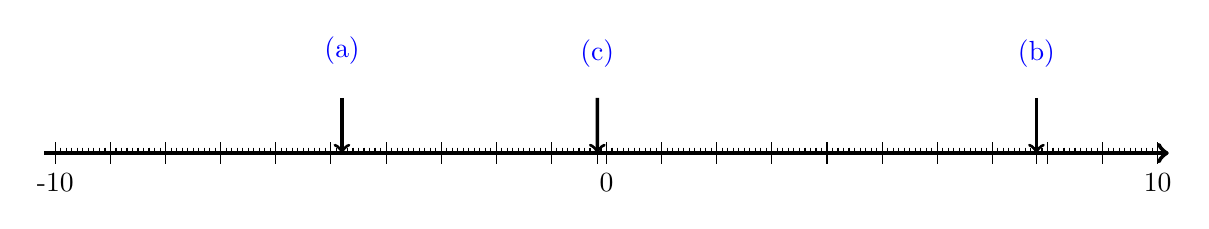
\begin{tikzpicture}[scale=0.7]
  \draw[->,ultra thick] (-10.2,0) -- (10.2,0);
  \foreach \i in {-10,-9,...,10} % numbers on line
    \draw ({10*\i/10},0.2) -- + (0,-0.4) node[below] {}; % tick and their labels
  \draw ({10*(-10)/10},0.2) -- + (0,-0.4) node[below] {-10};
  \draw (0,0.2) -- + (0,-0.4) node[below] {0};
  \draw ({10*(10)/10},0.2) -- + (0,-0.4) node[below] {10};
  \foreach \i in {-100,-99,...,100} % numbers on line
    \draw ({10*\i/100},0.1) -- + (0,-0.1) node[below] {}; % tick and their labels

  % réponses
\draw[very thick][->] (-4.8,1) -- (-4.8,0);
\draw[very thick][->] (7.8,1) -- (7.8,0);
\draw[very thick][->] (-0.1666,1) -- (-0.16666,0);
  \draw (-4.8,0.1) -- + (0,-0.1) node[above=1cm] {\color{blue}(a)};
 \draw (7.8,0.1) -- + (0,-0.3) node[above=1.1cm] {\color{blue}(b)};
 \draw (-0.1666,0.1) -- + (0,-0.3) node[above=1.1cm] {\color{blue}(c)};
\end{tikzpicture}}{1}
\end{resolu}


\begin{exo}{
Dessine une droite numérique (entre -10 et 10) et places-y le plus précisément possible les nombres suivants.
\[
a=6,25 \quad b=-\dfrac{7}{2} \quad c=\dfrac{3}{4} \quad d=-\dfrac{15}{4} \quad e=-2,35 \quad f=-\dfrac{25}{10} \quad g=\dfrac{8}{1} 
\]}
{1}\end{exo}

\begin{exo}{
Dessine une droite numérique (entre -4 et 1) et places-y le plus précisément possible les nombres suivants.
\[
a=-\dfrac{3}{1} \quad b=\dfrac{1}{4} \quad c=-\dfrac{2}{6} \quad d=\dfrac{1}{4} \quad e=-\dfrac{1}{5} \quad f=\dfrac{2}{6} \quad
g=-\dfrac{2}{5}
\]}
{1}\end{exo}

\begin{exo}{
Dessine une droite numérique (entre -2 et 2) et places-y le plus précisément possible les fractions suivantes.
\[
a=\dfrac{2}{20} \quad b=-\dfrac{7}{10} \quad c=-\dfrac{4}{5} \quad d=\dfrac{7}{5} \quad e=\dfrac{5}{10} \quad f=-\dfrac{3}{2}
\]}
{1}\end{exo}

%Amplifications et simplifications
\begin{exof}{NO106}{35}{3}
\end{exof}
\begin{exof}{NO107}{35}{3}
\end{exof}


\begin{resolu}{Comparaison}{ Compare ces nombres en utilisant le signe approprié. 
\begin{tasks}(2)
	\task
	$\dfrac{2}{3} \ldots < \ldots \dfrac{4}{3}$ 
    \task 
  $-\dfrac{2}{3} \ldots > \ldots -\dfrac{4}{3}$
\task $0,4 \ldots=\ldots \dfrac{4}{10}$
\task  $-\dfrac{8}{9}\ldots>\ldots-\dfrac{3}{2}$ 
\end{tasks}
}{1}
\end{resolu}


\begin{exop}{
Compare ces nombres en utilisant le signe approprié. 
\begin{tasks}(2)
	\task $\dfrac{2}{3}\ldots \ldots \dfrac{4}{3} $
	\task $\dfrac{4}{3}\ldots \ldots \dfrac{3}{4} $
    \task $-6\ldots \ldots \dfrac{1}{6} $
	\task $-\dfrac{7}{5}\ldots \ldots \dfrac{8}{5} $
	\task $\dfrac{2}{4}\ldots \ldots \dfrac{4}{2} $
    \task $\dfrac{54}{16}\ldots \ldots -\dfrac{45}{16} $
	\task $\dfrac{182}{13}\ldots \ldots \dfrac{1802}{13} $
 \task $\dfrac{154}{125}\ldots \ldots \dfrac{158}{189} $
\end{tasks}
}{1}
\end{exop}

\begin{exop}{
Compare ces nombres en utilisant le signe approprié. 
\begin{tasks}(2)
\task $-\dfrac{4}{5}\ldots \ldots \dfrac{4}{5} $
\task $-\dfrac{182}{15}\ldots \ldots \dfrac{182}{15} $
     \task $-\dfrac{7}{14}\ldots \ldots -\dfrac{5}{14} $
	\task $-\dfrac{30}{45}\ldots\ldots 
 -\dfrac{31}{45}$
	\task $-\dfrac{3}{7}\ldots \ldots -\dfrac{3}{11}$
   \task $-\dfrac{11}{5}\ldots \ldots -\dfrac{9}{5} $
 \task $0,2 \ldots \ldots \dfrac{2}{10} $
	\task $-\dfrac{7}{10}\ldots \ldots -\dfrac{3}{5} $
\end{tasks}
}{1}
\end{exop}

\begin{exop}{
Compare ces nombres en utilisant le signe approprié. 
\begin{tasks}(2)
	\task $-\dfrac{3}{4}\ldots \ldots -\dfrac{13}{16} $
    \task $-\dfrac{7}{4}\ldots \ldots -\dfrac{5}{3} $
	\task $\dfrac{8}{12}\ldots \ldots \dfrac{19}{24} $
	\task $-\dfrac{7}{4}\ldots \ldots -\dfrac{5}{3} $

\end{tasks}
}{2}
\end{exop}

%additions et soustrations de fractions
\begin{exof}{NO149}{46}{3}
\end{exof}
\begin{exof}{NO150}{46}{3}
\end{exof}
\begin{exof}{NO151}{47}{3}
\end{exof}
\begin{exof}{NO152}{48}{3}
\end{exof}

\begin{resolu}{Multiplication de deux fractions}{Calcule ces produits et rends le résultat sous la forme d'une fraction irréductible ou d'un entier.
\begin{tasks}
	\task  \begin{expli}
		 &\dfrac{4}{8}\cdot \dfrac{2}{3}=\dfrac{4 \cdot 2}{8 \cdot 3} & \text{On multiplie les numérateurs entre eux}\\ && \text{et on multiplie les dénominateurs entre eux. }\\

				 \vspace{0.4em}
				 &=\dfrac{8}{24}&\text{On obtient le produit de 4 par 2 au numérateur}\\
     &&\text{et de 8 par 3 au dénominateur.}\\
				&=\dfrac{1}{3} &\text{On donne le résultat sous la forme}\\
				&&\text{d'un entier ou d'une fraction irréductible.}
\end{expli}
\task  \begin{expli}
 &\dfrac{4}{-3}\cdot \dfrac{3}{4} = \dfrac{4 \cdot 3}{(-3)\cdot4} &\text{On multiplie les numérateurs entre eux}\\ && \text{et on multiplie les dénominateurs entre eux. }\\

				 \vspace{0.4em}
				 &=\dfrac{12}{-12} &\text{On obtient le produit de 4 par 3 au numérateur}\\
				&&\text{et le produit de -3 par 4 au dénominateur.}\\
    &=-\dfrac{12}{12} &\text{On sort le signe négatif de la fraction.}\\

             &=-1 &\text{On donne le résultat sous la forme}\\
              &&\text{d'un entier ou d'une fraction irréductible.}
\end{expli}
\end{tasks}
}{3}
\end{resolu}
\newpage

\begin{exop}{
Calcule ces produits et rends le résultat sous la forme d'une fraction irréductible ou d'un entier.
\begin{tasks}(2)
	\task $\dfrac{3}{7}\cdot \dfrac{6}{5}=$
    \task $\dfrac{8}{7}\cdot \dfrac{2}{3}=$
	\task $\dfrac{1}{2}\cdot \dfrac{3}{5}=$
	\task $\dfrac{2}{4}\cdot \dfrac{5}{7}=$
    \task $\dfrac{7}{3}\cdot \dfrac{5}{2}=$
	\task $\dfrac{6}{1}\cdot \dfrac{6}{7}=$
	\task $\dfrac{7}{12}\cdot \dfrac{5}{2}=$
	\task $\dfrac{3}{11}\cdot \dfrac{16}{5}=$
\end{tasks}
}{3}
\end{exop}

\begin{exop}{
Calcule ces produits et rends le résultat sous la forme d'une fraction irréductible ou d'un entier.
\begin{tasks}(2)
	\task $\dfrac{-3}{7}\cdot \dfrac{-3}{5}=$
    \task $\dfrac{6}{-7}\cdot \dfrac{1}{3}=$
	\task $\dfrac{-1}{-2}\cdot \dfrac{-3}{5}=$
	\task $\dfrac{2}{3}\cdot \dfrac{-5}{7}=$
    \task $\dfrac{4}{3}\cdot \dfrac{-5}{2}=$
	\task $\dfrac{-12}{5}\cdot \dfrac{-2}{5}=$
\end{tasks}
}{3}
\end{exop}

\newpage
\begin{resolu}{Multiplication de deux fractions avec simplification}{Simplifie ces fractions, puis calcule ces produits. Rends le résultat sous la forme d'une fraction irréductible ou d'un entier.
\begin{tasks}
	\task  \begin{expli}
		 &\dfrac{8}{7}\cdot \dfrac{14}{5}=\dfrac{8 \cdot 14}{7 \cdot 5}  & \text{On multiplie les numérateurs entre eux}\\ && \text{et on multiplie les dénominateurs entre eux. }\\

				 \vspace{0.4em}
				 &=\dfrac{8 \cdot 14}{5 \cdot 7} &\text{On réorganise les facteurs.}\\
     &&\text{afin de pouvoir simplifier la fraction.}\\
\vspace{0.5 cm}
				&=\dfrac{8\cdot2}{5\cdot1} &\text{On simplifie la fraction par 7.}\\
				&=\dfrac{16}{5} &\text{On effectue le produit et on rend le résultat}\\ &&\text{sous la forme d'une fraction irréductible.}
\end{expli}
	\task  \begin{expli}
		 &\dfrac{3}{5}\cdot \dfrac{15}{6}=\dfrac{3 \cdot 15}{5 \cdot 6}  & \text{On multiplie les numérateurs entre eux}\\ && \text{et on multiplie les dénominateurs entre eux. }\\

				 \vspace{0.4em}
				 &=\dfrac{3 \cdot 15}{6 \cdot 5} &\text{On réorganise les facteurs.}\\
     &&\text{afin de pouvoir simplifier la fraction}\\
\vspace{0.5 cm}
				&=\dfrac{1\cdot15}{2\cdot5} &\text{On simplifie la fraction par 3.}\\
    \vspace{0.5cm}
				&=\dfrac{1\cdot3}{2\cdot1}&\text{On simplifie la fraction par 5.}\\ 

    
             &=\dfrac{3}{2}
    &\text{On effectue le produit}\\
\end{expli}
\end{tasks}
}{3}
\end{resolu}

\begin{exop}{
Simplifie ces fractions, puis calcule ces produits. Rends le résultat sous la forme d'une fraction irréductible ou d'un entier.
\begin{tasks}(2)
	\task $\dfrac{8}{5}\cdot \dfrac{10}{1}=$
    \task $\dfrac{3}{9}\cdot \dfrac{2}{8}=$
	\task $\dfrac{10}{15}\cdot \dfrac{8}{4}=$
	\task $\dfrac{20}{7}\cdot \dfrac{21}{5}=$
    \task $\dfrac{7}{1}\cdot \dfrac{6}{7}=$
	\task $\dfrac{16}{11}\cdot \dfrac{44}{48}=$
	\task $\dfrac{7}{9}\cdot \dfrac{3}{14}=$
	\task $\dfrac{9}{2}\cdot \dfrac{10}{5}=$
\end{tasks}
}{3}
\end{exop}

\begin{exop}{
Simplifie ces fractions, puis calcule ces produits. Rends le résultat sous la forme d'une fraction irréductible ou d'un entier.
\begin{tasks}(2)
	\task $\dfrac{-10}{27}\cdot \dfrac{3}{30}=$
    \task $\dfrac{4}{6}\cdot \dfrac{-1}{7}=$
	\task $\dfrac{-8}{-16}\cdot \dfrac{2}{3}=$
	\task $\dfrac{10}{-15}\cdot \dfrac{-14}{7}=$
    \task $\dfrac{7}{12}\cdot \dfrac{4}{8}=$
	\task $\dfrac{1}{-7}\cdot \dfrac{14}{2}=$
	\task $\dfrac{-24}{15}\cdot \dfrac{15}{24}=$
	\task $\dfrac{3}{8}\cdot \dfrac{-6}{-9}=$
\end{tasks}
}{3}
\end{exop}


\begin{resolu}{Multitplication d'un nombre entier et d'une fraction}{ Calcule ces produits et rends le résultat sous la forme d'une fraction irréductible ou d'un entier. 
\begin{tasks}
	\task  \begin{expli}
		 &6\cdot \dfrac{2}{3} = \dfrac{6}{1}\cdot\dfrac{2}{3} & \text{Le facteur (ici le nombre 6)}\\ && \text{ne multiplie que le numérateur de la fraction. }\\

				 \vspace{0.4em}
				 &=\dfrac{12}{3} &\text{On obtient le produit de 2 par 6 au numérateur.}\\
				&=4 &\text{On donne le résultat sous la forme}\\
				&&\text{d'un entier ou d'une fraction irréductible.}
\end{expli}
\task  \begin{expli}
 & -4\cdot \dfrac{3}{5} = \dfrac{-4 \cdot 3}{5}  & \text{Le facteur (ici le nombre relatif -4)}\\ && \text{ne multiplie que le numérateur de la fraction. }\\

				 \vspace{0.4em}
				 &=\dfrac{-12}{5} &\text{On obtient le produit de -4 par 3 au numérateur.}\\
				&&\text{On donne le résultat sous la forme}\\
				&&\text{d'un entier ou d'une fraction irréductible.}
\end{expli}
\end{tasks}
}{3}
\end{resolu}

\begin{exop}{
Calcule ces produits et rends le résultat sous la forme d'une fraction irréductible ou d'un entier.
\begin{tasks}(2)
	\task $7\cdot \dfrac{1}{7}=$
    \task $\dfrac{3}{4}\cdot5=$
	\task $0\cdot \dfrac{19}{17}=$
	\task $2\cdot \dfrac{5}{8}=$
    \task $\dfrac{5}{2}\cdot2=$
	\task $3\cdot \dfrac{2}{3}=$
	\task $5\cdot \dfrac{1}{7}=$
	\task $11\cdot \dfrac{2}{22}=$
\end{tasks}
}{3}
\end{exop}

\begin{exop}{
Calcule ces produits et rends le résultat sous la forme d'une fraction irréductible ou d'un entier.
\begin{tasks}(2)
	\task $7\cdot \dfrac{-3}{5}=$
	\task $-2\cdot \dfrac{-19}{17}=$
	\task $2\cdot \dfrac{4}{-8}=$
    \task $\dfrac{12}{13}\cdot(-3)=$
	\task $0\cdot \dfrac{-2}{3}=$
	\task $25\cdot \dfrac{-1}{-5}=$
\end{tasks}
}{3}
\end{exop}

%multiplications
%156 - 161
\begin{exof}{NO157}{50}{3}
\end{exof}
\begin{exof}{NO158}{50}{3}
\end{exof}
\begin{exof}{NO159}{50}{3}
\end{exof}
\begin{exof}{NO160}{50}{3}
\end{exof}
\begin{exof}{NO161}{51}{1}
\end{exof}

%problèmes
\begin{resolu}{Problème}{Dans une école, $\dfrac{7}{10}$ des élèves mangent au réfectoire à midi. Parmi ceux-ci, $\dfrac{1}{4}$
sont végétariens. 
\begin{tasks}
    \task Quelle fraction d'élèves représente les élèves végétariens?
    \task Quel pourcentage cela représente-t-il?
\end{tasks}
\begin{tasks}
    

    \task $\dfrac{7}{10} \cdot \dfrac{1}{4} = \dfrac{7}{40}$
    \vspace{0.5cm}
    \task $\dfrac{7}{40}=0,175=17,5 \%$
\end{tasks}
}{3}
\end{resolu}

\begin{exo}{Dans une animalerie, $\dfrac{3}{4}$ des animaux sont des rongeurs. Parmis ces rongeurs, $\dfrac{5}{6}$ sont des lapins.
\begin{tasks}
    \task Quelle fraction d'animaux représente les lapins?
    \task Quel pourcentage cela représente-t-il?
\end{tasks}
}{3}   
\end{exo}

\begin{exo}{Un champ est cultivé avec $\dfrac{1}{4}$ de roses, $\dfrac{3}{8}$ de jonquilles et $\dfrac{6}{16}$ de tulipes. Cette année, le mauvais temps a détruit le tiers des tulipes.
\begin{tasks}
    \task Quelle fraction du champ les tulipes détruites représentent-elles?
    \task Quelle fraction du champ représente les tulipes intactes? 
    \task Quel pourcentage les tulipes intactes représentent-elles alors ?
\end{tasks}
}{3}   
\end{exo}

\begin{exol}{NO163}{46}{3}
\end{exol}
\begin{exol}{NO164}{46}{3}
\end{exol}
\begin{exol}{NO165}{46}{3}
\end{exol}



\begin{resolu}{Division de fractions}{ Calcule ces quotients et rends le résultat sous la forme d'une fraction irréductible ou d'un entier. 
\begin{tasks}
	\task  \begin{expli}
 \vspace{0.6cm}
		 &\dfrac{2}{3}\div \dfrac{1}{3} \\
				 \vspace{0.6cm}
				 &=\dfrac{2}{3} \cdot  \dfrac{3}{1} &\text{On inverse la deuxième fraction.}\\
     \vspace{0.6cm}
				&=\dfrac{2 \cdot 3}{3\cdot1} & \text{On effectue le produit des deux fractions.}\\
                \vspace{0.6cm}
                &=\dfrac{6}{3}\\
                
                &=2
    &\text{On donne le résultat sous la forme}\\
				&&\text{d'un entier ou d'une fraction irréductible.}
\end{expli}
\task  \begin{expli}
 \vspace{0.6cm}
		 & \dfrac{3}{5}\div \dfrac{1}{4} \\
				 \vspace{0.6cm}
				 &=\dfrac{3}{5} \cdot \dfrac{4}{1} &\text{On inverse la deuxième fraction.}\\
     \vspace{0.6cm}
				&=\dfrac{3 \cdot 4}{5\cdot1} & \text{On effectue le produit des deux fractions.}\\
       
                &=\dfrac{12}{5}
    &\text{On donne le résultat sous la forme}\\
				&&\text{d'un entier ou d'une fraction irréductible.}
\end{expli}
\end{tasks}
}{3}
\end{resolu}

\begin{exop}{
Calcule ces quotients et rends le résultat sous la forme d'une fraction irréductible ou d'un entier.
\begin{tasks}(2)
	\task $\dfrac{3}{7}\div \dfrac{9}{3}=$
    \task $\dfrac{8}{12}\div \dfrac{2}{3}=$
	\task $\dfrac{5}{3}\div \dfrac{2}{7}=$
	\task $\dfrac{1}{2}\div \dfrac{2}{1}=$
    \task $\dfrac{12}{6}\div \dfrac{4}{7}=$
	\task $\dfrac{7}{10}\div \dfrac{14}{5}=$
	\task $\dfrac{12}{9}\div \dfrac{8}{12}=$
	\task $\dfrac{1}{3}\div \dfrac{32}{6}=$
\end{tasks}
}{3}
\end{exop}

\begin{exop}{
Après avoir simplifié la fraction, calcule ces quotients et rends le résultat sous la forme d'une fraction irréductible ou d'un entier.
\begin{tasks}(2)
	\task $\dfrac{8}{24}\div \dfrac{32}{6}=$
    \task $\dfrac{6}{5}\div \dfrac{2}{2}=$
	\task $\dfrac{36}{48}\div \dfrac{12}{8}=$
	\task $\dfrac{7}{10}\div \dfrac{14}{5}=$
    \task $\dfrac{20}{16}\div \dfrac{5}{8}=$
	\task $\dfrac{8}{2}\div \dfrac{3}{9}=$
	\task $\dfrac{5}{10}\div \dfrac{15}{5}=$
	\task $\dfrac{7}{14}\div \dfrac{9}{6}=$
\end{tasks}
}{3}
\end{exop}

\begin{exop}{
Calcule ces quotients et rends le résultat sous la forme d'une fraction irréductible ou d'un entier.
\begin{tasks}(2)
	\task $\dfrac{-5}{7}\div \dfrac{-1}{3}=$
    \task $\dfrac{2}{-6}\div \dfrac{-2}{3}=$
	\task $\dfrac{-3}{4}\div \dfrac{1}{7}=$
	\task $\dfrac{7}{2}\div \dfrac{-2}{4}=$
    \task $\dfrac{-3}{5}\div \dfrac{-2}{5}=$
	\task $\dfrac{3}{9}\div \dfrac{-4}{6}=$
	\task $\dfrac{2}{-9}\div \dfrac{-2}{6}=$
	\task $\dfrac{2}{3}\div \dfrac{3}{6}=$
\end{tasks}
}{3}
\end{exop}

\begin{exop}{
Calcule et rends le résultat sous la forme d'une fraction irréductible ou d'un entier.
\begin{tasks}(2)
	\task $\dfrac{3}{2}\cdot \dfrac{1}{3}=$
    \task $\dfrac{3}{12}\div \dfrac{2}{4}=$
	\task $\dfrac{5}{3}\cdot \dfrac{2}{5}=$
	\task $\dfrac{10}{2}\div \dfrac{12}{10}=$
    \task $\dfrac{2}{6}\cdot \dfrac{4}{3}=$
	\task $\dfrac{4}{15}\div \dfrac{1}{5}=$
	\task $\dfrac{2}{7}\cdot \dfrac{2}{3}=$
	\task $\dfrac{1}{2}\div \dfrac{3}{6}=$
\end{tasks}
}{3}

\begin{resolu}{Division d'une fraction par un nombre entier}{ Calcule ces quotients et rends le résultat sous la forme d'une fraction irréductible ou d'un entier. 
\begin{tasks}
	\task  \begin{expli}
 \vspace{0.6cm}
		 &\dfrac{2}{3}\div 6 = \dfrac{2}{3}\div \dfrac{6}{1}& \text{On met le nombre entier sous forme fractionnaire.}\\
				 \vspace{0.6cm}
				 &=\dfrac{2}{3} \cdot \dfrac{1}{6} &\text{On inverse la deuxième fraction.}\\
     \vspace{0.6cm}
				&=\dfrac{2 \cdot 1}{3\cdot6} & \text{On effectue le produit des deux fractions.}\\
                \vspace{0.6cm}
                &=\dfrac{2}{18}\\
                
                &=\dfrac{1}{9}
    &\text{On donne le résultat sous la forme}\\
				&&\text{d'un entier ou d'une fraction irréductible.}
\end{expli}
\task  \begin{expli}
 \vspace{0.6cm}
		 &7\div \dfrac{1}{4} = \dfrac{7}{1}\div \dfrac{1}{4}& \text{On met le nombre entier sous forme fractionnaire.}\\
				 \vspace{0.6cm}
				 &=\dfrac{7}{1} \cdot  \dfrac{4}{1} &\text{On inverse la deuxième fraction.}\\
     \vspace{0.6cm}
				&=\dfrac{7 \cdot 4}{1\cdot1} & \text{On effectue le produit des deux fractions.}\\
                \vspace{0.6cm}
                &=\dfrac{28}{1}\\
                
                &=28
    &\text{On donne le résultat sous la forme}\\
				&&\text{d'un entier ou d'une fraction irréductible.}
\end{expli}
\end{tasks}
}{3}
\end{resolu}

\begin{exop}{
Calcule ces quotients et rends le résultat sous la forme d'une fraction irréductible ou d'un entier.
\begin{tasks}(2)
	\task $10\div \dfrac{1}{15}=$
    \task $2\div \dfrac{4}{2}=$
	\task $9\div \dfrac{1}{15}=$
	\task $\dfrac{3}{7}\div 5=$
    \task $\dfrac{5}{3}\div 6=$
	\task $\dfrac{1}{4}\div 2=$
	\task $\dfrac{14}{3}\div 9=$
	\task $5\div \dfrac{9}{4}=$
\end{tasks}
}{3}
\end{exop}
\newpage
\begin{exop}{
Calcule ces quotients et rends le résultat sous la forme d'une fraction irréductible ou d'un entier.
\begin{tasks}(2)
	\task $11\div \dfrac{-2}{3}=$
    \task $-13\div \dfrac{1}{2}=$
	\task $-3\div \dfrac{-2}{7}=$
	\task $\dfrac{-2}{5}\div -4=$
    \task $\dfrac{-3}{6}\div -2=$
	\task $\dfrac{3}{4}\div -5=$
	\task $\dfrac{-11}{5}\div -5=$
	\task $-7\div \dfrac{4}{2}=$
\end{tasks}
}{3}
\end{exop}
\end{exop}
\begin{exof}{NO171}{52}{3}
\end{exof}
\begin{exof}{NO172}{52}{3}
\end{exof}


\begin{exol}{NO173}{47}{3}
\end{exol}

\begin{exol}{NO174}{47}{3}
\end{exol}

\begin{exol}{NO175}{47}{3}
\end{exol}




\begin{resolu}{Puissances et fractions}{Calcule ces produits et rends le résultat sous la forme d'une fraction irréductible ou d'un entier.
\begin{tasks}
	\task  \begin{expli}
  \vspace{0.5cm}
		 & \left( \dfrac{4}{8} \right)^2=\dfrac{4}{8} \cdot \dfrac{4}{8}  & \text{On multiplie les fractions.}\\

				 \vspace{0.4cm}
				 &=\dfrac{16}{64}&\text{On obtient le produit de $4^2$ et de $8^2$.}\\
				&=\dfrac{1}{4} &\text{On donne le résultat sous la forme}\\
				&&\text{d'un entier ou d'une fraction irréductible.}
\end{expli}
\task  \begin{expli}
				 \vspace{0.5cm} 
 &\dfrac{4^2}{3} = \dfrac{4 \cdot 4}{3} &\text{On effectue l'exponentiation au numérateur.}\\ 

				 \vspace{0.5cm}
				 &=\dfrac{16}{3} &\text{On obtient le produit de 4 par 4 au numérateur.}\\

\end{expli}
\end{tasks}
}{3}
\end{resolu}
\newpage
\begin{exop}{
Calcule et rends le résultat sous la forme d'une fraction irréductible ou d'un entier.
\begin{tasks}(2)
	\task $\left(\dfrac{3}{12} \right)^2=$
    \task $\dfrac{3^2}{12}=$
	\task $\left(\dfrac{3}{2} \right)^3=$
	\task $\dfrac{4}{5^2}=$
    \task $\left(\dfrac{4}{5} \right)^2=$
	\task $\dfrac{2}{6^2}=$
	\task $\left(\dfrac{1}{2} \right)^3=$
	\task $\dfrac{4^2}{8}=$
\end{tasks}
}{3}
\end{exop}

%problèmes 173-175



%problèmes mélangés 180-181 183-188


\begin{resolu}{Priorité des opérations}{Calcule et rends le résultat sous la forme d'une fraction irréductible ou d'un entier.
\begin{tasks}
	\task  \begin{expli}
 \vspace{0.4cm}
		 & \left( \dfrac{4}{8} \right)^2 \cdot \dfrac{1}{2}=\dfrac{4\cdot4}{8\cdot 8} \cdot \dfrac{1}{2}  & \text{On effectue la puissance en premier.}\\

				 \vspace{0.4cm}
				 &=\dfrac{16}{64}\cdot \dfrac{1}{2}&\text{puis on effectue le produit}\\
       \vspace{0.5cm}
				&=\dfrac{16}{128}\\
   
   & =\dfrac{1}{8} &\text{On donne le résultat sous la forme}\\
				&&\text{d'un entier ou d'une fraction irréductible.}
\end{expli}
\task  \begin{expli}
\vspace{0.4cm}
 &\dfrac{4^2}{3}+\dfrac{1}{2} = \dfrac{4 \cdot 4}{3} + \dfrac{1}{2} &\text{On effectue l'exponentiation au numérateur.}\\ 

				 \vspace{0.4cm}
				 &=\dfrac{16}{3}+\dfrac{1}{2} \\
     
 \vspace{0.4cm}
				 &=\dfrac{32}{6}+\dfrac{3}{6} &\text{On amplifie les factions pour les additionner.}\\
      \vspace{0.4cm}
				 &=\dfrac{35}{6}
\end{expli}
\end{tasks}
}{3}
\end{resolu}

\begin{exo}{
Calcule et donne le résultat sous la forme d'une fraction irréductible ou d'un entier.
\begin{tasks}(2)
	\task $\dfrac{3}{4}+\dfrac{2}{5} \cdot \dfrac{15}{7}=$
    \task $\dfrac{6}{5} \div \dfrac{2}{3}+\dfrac{1}{4}=$
	\task $\left(\dfrac{8}{5}-\dfrac{2}{3} \right)\cdot \dfrac{4}{3}=$
	\task $\dfrac{5}{15}\div\left(\dfrac{2}{3}+\dfrac{1}{6} \right)=$
    \task $\left(\dfrac{3}{4}+\dfrac{1}{3}\div\dfrac{13}{2} \right)^2=$
	\task $\dfrac{8}{2}\cdot\dfrac{3}{2}-\left(-\dfrac{1}{4} \right)=$
	\task $\left(-\dfrac{1}{5} \right)^2\cdot\dfrac{3}{4}\cdot\dfrac{1}{2}=$
	\task $\left(-\dfrac{2}{3}\right)+\left(-\dfrac{5}{2}\right)\cdot3=$
    \task $\left(\dfrac{3}{4}+\dfrac{1}{3}\right)\div \dfrac{12}{5}=$
    \task $\dfrac{2}{3}-\left(\dfrac{1}{2}+\dfrac{3}{5}\right)=$
\end{tasks}
}{3}
\end{exo}

\newpage
\begin{exo}{
Calcule et donne le résultat sous la forme d'une fraction irréductible ou d'un entier.
\begin{tasks}(2)
	\task $\dfrac{3}{10}\cdot \dfrac{5}{6} + \dfrac{2}{7}\cdot \dfrac{21}{6}=$
    \task $\left(0,4-\dfrac{3}{10}\right)\cdot\dfrac{20}{3}=$
	\task $\left(\dfrac{3}{2}+\dfrac{1}{8} \right)\div \left(\dfrac{1}{8}-\dfrac{2}{5}\right)=$
	\task $\left(-\dfrac{3}{2}\right)- 5\cdot\dfrac{3}{4}=$
    \task $\dfrac{7}{4}\cdot\dfrac{8}{3}+\dfrac{1}{5} \cdot \dfrac{25}{2}=$
	\task $\dfrac{8}{7}\div\left(\dfrac{1}{2}+\dfrac{1}{3} \right)=$
	\task $\left(\dfrac{2}{3} \right)^3 \cdot \dfrac{4}{3}=$
	\task $\left(\dfrac{5}{4}-\dfrac{1}{3}\right)\cdot\left(\dfrac{1}{2}+\dfrac{3}{5}\right)=$
    \task $6-\left(\dfrac{3}{3}+\dfrac{7}{8}\right)=$
    \task $\left(\dfrac{3}{4}+\dfrac{2}{3}\right)^2=$
\end{tasks}
}{3}
\end{exo}

\begin{exof}{NO176}{55}{3}
\end{exof}
\begin{exof}{NO177}{55}{3}
\end{exof}
\begin{exof}{NO178}{56}{3}
\end{exof}
\begin{exof}{NO179}{56}{3}
\end{exof}

\begin{exol}{NO153}{44}{3}
\end{exol}

\begin{FLP}{53}{3}
\end{FLP}
\end{document}
